% !TEX encoding = UTF-8 Unicode
%!TEX root = thesis.tex
% !TEX spellcheck = en-US
%%=========================================
\addcontentsline{toc}{section}{Preface}
\section*{Preface}

The following is my master's thesis, written at the NTNU Faculty of Natural Sciences as a  part of my master's degree in Applied Physics and Mathematics. Starting in January and spanning over the 2018 spring semester, the accompanying project work was carried out for SINTEF Ocean and supervised by Associate Professor Tor Nordam.

Having previously cooperated with Assoc. Prof. Nordam, considering interpolator performance in relation to identification of hyperbolic Lagrangian coherent structures (LCSs) in two dimensions, Tor approached me and fellow student Arne Magnus Tveita Løken with the present problem statement. Acknowledging the complexities of LCS identification in three dimensions, this project has been carried out in cooperation with Arne. Although writing separate theses, it should be noted that we devised all methods and computed all results collaboratively. The guidance and support, as well as enthusiastic disposition, of Associate Professor Nordam has also been a constant source of help, inspiration, and motivation throughout the process

The intended audience of this report possesses a level of knowledge of physics and mathematics corresponding to that expected at a master's level physics program. While in-depth knowledge of finite strain theory and numerical analysis could prove helpful, all advanced methods and concepts are explained prior to application. The code used to produce the results presented in this thesis is available at github.\footnote{https://github.com/arnemagnus/3d\_lcs}

\begin{center}
Trondheim, 2018-06-11\\[1pc]
\begin{figure}[h!]
\centering
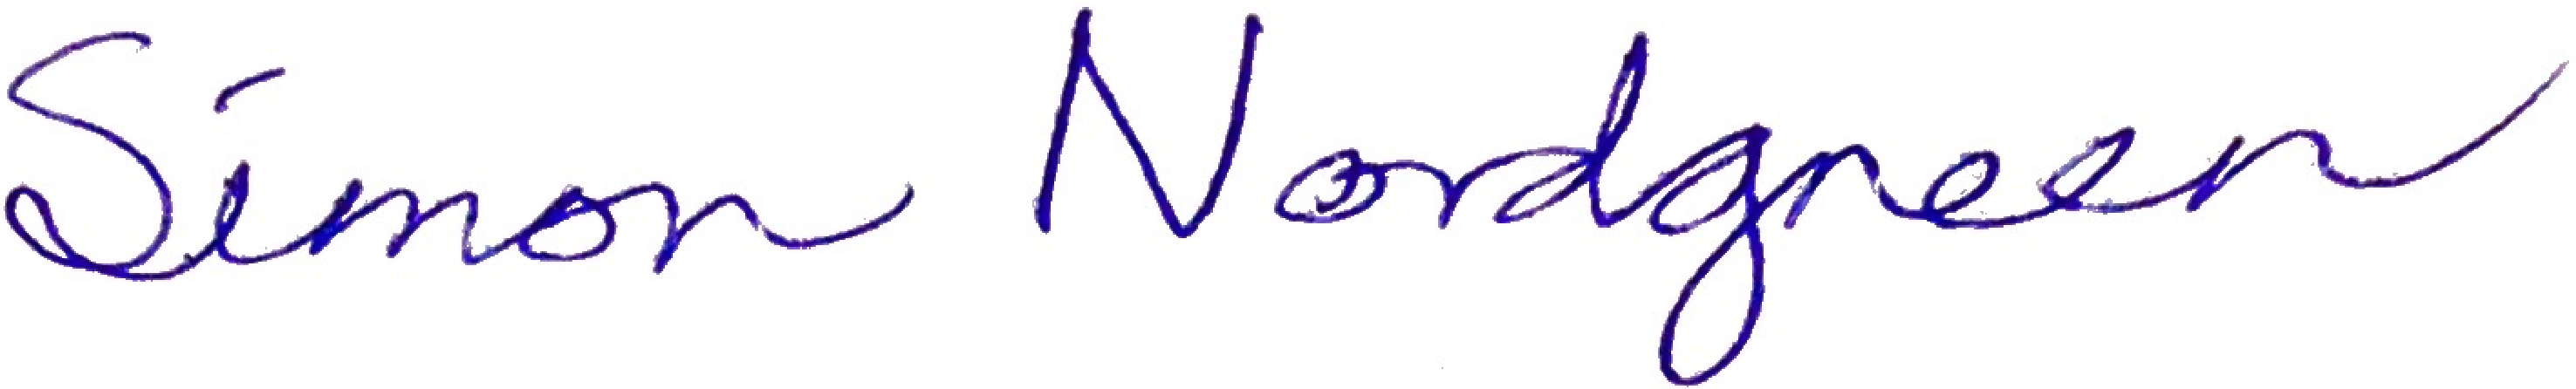
\includegraphics[totalheight=1cm]{fig/signature_cropped.pdf}
\end{figure}

%(Your signature)\\[1pc]
Simon Nordgreen
\end{center}